\documentclass[conference]{IEEEtran}
\IEEEoverridecommandlockouts
% The preceding line is only needed to identify funding in the first footnote. If that is unneeded, please comment it out.
\usepackage{cite}
\usepackage{amsmath,amssymb,amsfonts}
\usepackage{algorithmic}
\usepackage{graphicx}
\usepackage{textcomp}
\usepackage{xcolor}
\usepackage{listings}
\usepackage{pgfplotstable}
\usepackage[]{algorithm2e}
\usepackage{url}
\def\BibTeX{{\rm B\kern-.05em{\sc i\kern-.025em b}\kern-.08em
    T\kern-.1667em\lower.7ex\hbox{E}\kern-.125emX}}
\begin{document}

\title{Extended Generative Adversarial Networks}

\author{\IEEEauthorblockN{John Hancock}
\IEEEauthorblockA{\textit{College of Engineering and Computer Science} \\
\textit{Florida Atlantic University}\\
Boca Raton, United States of America\\
jhancoc4@fau.edu}}


\maketitle

\begin{abstract}
In this work we explore extending generative adversarial networks (GAN's).
Authors of previous research document GAN's with one generator and one
discriminator. In this work we explore GAN's with more than one generator or
discriminator.  We term the type of multiple generative adversarial networks in
this work \textbf{chained generative adversarial networks}.  We investigate the
performance of these extended GAN's, with a special focus on the accuracy of
discriminators in these chained generative adversarial networks.
\end{abstract}

\begin{IEEEkeywords}
generative adversarial networks, gan, neural networks, deep learning
\end{IEEEkeywords}

\section{Introduction}

In this work our goal is to investigate the behavior of generative adversarial
networks when one generative adversarial network uses the output of a previous
generative adversarial network for input.  Specifically we design a way to take
the output of a base generative adversarial network, that is the output of both
the generator and the discriminator of the base generative adversarial network,
and use that as the input for a subsequent generative adversarial network.  We
then extend this iterative use of the output of previous generative adversarial
networks 5 times, and investigate the changes in the performance of the
subsequent generative adversarial networks, as well as the quality of the
artifacts that the generative adversarial networks produce.

Generative adversarial networks are pairs of neural networks that generate
artifacts in an iterative fashion.  Goodfellow \textit{et al}. Introduce
Generative adversarial networks in their paper, ``Generative adversarial nets''
\cite{gan}.  This paper describes a stable system comprised of a generator and a
discriminator where the generator iteratively learns to create artifacts that
the discriminator iteratively learns to discriminate whether the current input
it sees is an artifact from the generator, or an instance of some dataset. 

In \cite{gan} Goodfellow \textit{et al}. Give a strong formal justification for
the stability of their design, which inspired subsequent researchers to find
good implementations of their design.  One successful implementation is from
Radford, Metz, and Chintala expose in \cite{repLearnDcgan}.  This design is
referenced in other works such as \cite{lsgan}, the so-called least squares deep
convolutional generative adversarial network.  There are many other bodies of
research that exploit the architecture in \cite{repLearnDcgan}, and we see how
the initial idea of Goodfellow \textit{et al.} is extensible in and of itself,
but also that subsequent refinements of it also take on lives of their own.

Alternatives to generative adversarial networks for generating artifacts that
would appear to be instances of a dataset include Deep Boltzman Machines
\cite{boltzmann}, and variational autoencoders \cite{varbayes}.

The inspiration for this work is the notion that a generator, when armed with
the previous result of another generator training to create the same kinds of
artifacts might be able to create a better quality artifact.  We find that this
is not the case.  However, our results show that some information may be
preserved because when we pass the output of a previous generator to a
subsequent generator, along with the value of the loss function associated with
the value from that generator, then we find some noticeable impact on the
accuracy of the discriminator in the subsequent generative adversarial network.

At the time of this writing, we do not find a similarly structured collection of
generative adversarial networks that we we propose in the architecture we review
in this work.

Additionally we would like to point out to the reader early on that the source
code for the architecture and results we cover in this work is available with
details in reference \cite{jhcgan}.

\section{Related Work}

The seminal work on generative adversarial networks is the paper entitled, 
``Generative Adversarial Nets'' \cite{gan}.  In this work, Goodfellow \textit{et
al.} give the formal basis for generative adversarial networks. They prove
that under the proper conditions, a system of neural networks comprised of a 
generator and a discriminator will converge to a stable state.  The
discriminator has two sources of input: the output of the generator, and the
instances of some dataset.  The discriminator outputs a probability that the
input it received is from the dataset.  The generator
and the discriminator are locked in an adversarial relationship in the sense
that the generator's optimizer is driven using a loss function that incurs a
high loss for when the discriminator gives a low probability that its input is
from the dataset.  At the same time the discriminator's own optimizer uses a
loss function that incurs a high loss when the discriminator gives a probability 
that its input is from the generator when it is actually from the dataset, and
vice-versa.  The experiments we perform in this work show that it could be
possible to chain generative adversarial networks in such a way that the
ultimate discriminator is always capable of determining where its input is
coming from, \textit{i.e.} the generator, or the dataset.  We are not capable of
providing a formal derivation for our empirical results at this time, so we do
not state for certain that this is the case.

The formal derivation of the stability of generative adversarial networks that
Goodfellow \textit{et al.} find in \cite{gan}, we believe, gave researchers
confidence in pursuing implementations inspired by the idea that one could
employ neural networks to create artifacts that sufficiently resemble instances
of some dataset.  A milestone in the evolution of generative adversarial network
implementations is the work of Radford, Metz, and Chintala, in their work, 
``Unsupervised Representation Learning with Deep Convolutional Generative
Adversarial Networks'' \cite{repLearnDcgan}.  This work provides an architecture for
generative adversarial networks using convolutional neural networks.  Many
researchers employ or cite this architecture in the work.  Examples
include:Fussell and Moews in \cite{galaxy}, who incorporate Radfor, Metz,and 
Chintala's design into generative adversarial networks for generating images of
galaxies.   Goodfelow \textit{et al.} mention that Radford, Metz, and Chintala's 
work in \cite{repLearnDcgan} is notable for its performance due to their architecture,
and hyperparameter choices in their deep learning text,
\cite{deepLearnBookGenCh}.  In our experiments we use a Keras implemenation of
Radford, Metz, and Chintala's deep convolutional generative adversarial 
network as a basic building block.   We found the keras implementation of 
Radford, Metz, and Chinatala's generative adversarial network design in
\cite{kerasdcgan}.

A subsequent refinement of \cite{repLearnDcgan} is the least squares generative
adversarial network \cite{lsgan}. In this work Mao \textit{et al.} leverage
Radford, Metz, and Chintala's architecture with a least squares loss function in 
the discriminator to produce higher quality artifacts from their generative
adversarial networks. We feel that the existence of derivative works from the 
architecture that Radford, Metz, and Chintala give indicates that their
architecture is a good starting point for exploratory work in generative
adversarial networks, and another reason we chose to use their architecture as
a starting point for our design.

We find much interest in using generative adversarial networks as transformative
agents that manipulate their inputs into outputs that retain some aspects of
their inputs; however, the output is unique in some way that has aesthetic
appeal and appears in some sense natural.  A popular application of generative
adversarial networks in this domain is the pix2pix software that Isola, Zhu,
Zhou, and Efros cover in \cite{pix2pix}.  

In \cite{pix2pix} the authors show examples of applications of GAN's to produce
realistic images of things that do not exist, based on actual images, such that
the produced images do not appear to be synthetic to human observers.  Even though 
this may be the case, we posit that the result of the experiment we perform
below shows that one should be capable of training a series of discriminators
that would be able to distinguish the generated output from instances of some
dataset that the generated output is meant to resemble.  Often times, this point
will be moot because the generated output is not intended to substitute for
actual instances of some dataset.  Nevertheless there is perhaps an application
of our method for the purposes of forgery detection.


Researchers in the field of generative adversarial networks have turned their
attention to leveraging the output of generators as inputs to successive stages
of artifact generation. 

We found recent interest in the medical application of generative adversarial 
networks to creating simulated images of scar tissue in human hearts in
\cite{scargan}.  In this work Lau \textit{et al.} use a first GAN to generate
the shape of the scar tissue in an image, and then a second GAN to generate a 
refined image that uses the first image as input.

Further research along the lines of Lau \textit{et al.}'s work lead us to the
discovery of the StackGAN architecture of Zhang \textit{et al.} \cite{stackgan}.
The StackGAN architecture is similar to the architecture Lau et. al. propose.  
It consists of a stage-I generative adversarial network and a stage-II
generative adversarial network.  The stage-I generative adversarial network 
generates a basic image, and the stage-II generative adversarial network
generates a refinement of the image coming from stage-I.  Our work differs from
Zhang \textit{et al.}'s work in that we are interested in the behavior of the
discriminator, and not the quality of the artifacts that the generator produces.

However, our work indicates that if we augment the loss function of the
discriminator involved in generating the first image with the value of the loss
function for generating the first image, and use that as input for a subsequent
chain of generators then eventually the discriminators will be capable of
distinguishing actual versus generated images with a high degree of accuracy.
At this time we do not have a formal justification for this belief, but only the
empirical result of our experiment.

Research for related work involving generative adversarial networks that use
inputs other than pure noise brings us to the domain of conditioned generative
adversarial networks \cite{cgan}.  Since Goodfellow \textit{et al.} define
generative adversarial networks as using vectors of noise as inputs we felt it
important to confirm that researchers explore using different kinds of inputs
for generators.  Mizra and Osindero in \cite{cgan} deliver a proof-of-concept
work that adds labels to both the generator and discriminator inputs.  The
resulting generative adversarial network, after training, has a generator that
is then capable of producing artifacts with labels as conditions.  In
\cite{cgan} Mizra and Osindero give a table of generated MNIST \cite{mnist}
digits.  The table shows that when their generative adversarial network is 
conditioned with a particular label as part of its input, it will produce an
artifact that resembles the class of instances of the dataset that the label
is a member of.  We speculate that a formal justification for our result that
implies successive discriminators are more capable of classifying inputs as
generated, versus coming from an actual dataset, may stem from the notion that
we are giving a component of the previous discriminator's loss function value as
input to subsequent generators.  We feel this is similar to the notion of giving
data labels as inputs to the generator and discriminator.

After performing this research for related work, we did not find work that
exactly matches our procedure for linking generative adversarial networks.  We
find that the output of our chained generative adversarial networks is
unremarkable, however we feel the reader may wish to take note of the increased
accuracy of the series of discriminators that we find empirically.

\section{Chained generative adversarial networks}
This work is centered on a design for generative adversarial networks we call
\textbf{chained generative adversarial networks}.  The figure below illustrates
the architecture of a chained generative adversarial network at a high level.
\begin{figure}[htpb]
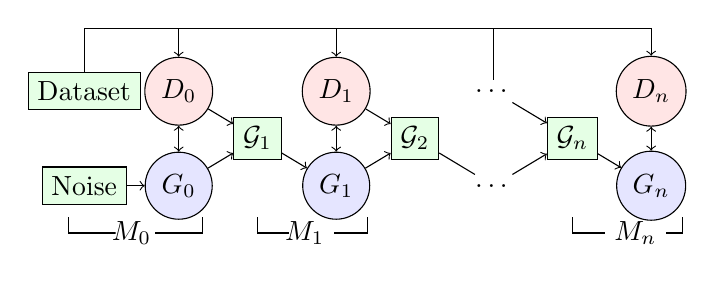
\begin{tikzpicture}
%style for generator node
\tikzstyle{gnode} = [circle, fill=blue!10, draw=black]

%style for discriminator node
\tikzstyle{dnode} = [circle, fill=red!10, draw=black]

%style for input box
\tikzstyle{inbox} = [rectangle, fill=green!10, draw=black]

%place nodes
\node[gnode](G0) at (0,0) {$G_{0}$};
\node[dnode](D0) at (0,1.2) {$D_{0}$};
\node(M0) at (-0.6, -0.6) {$M_{0}$};
\node[inbox] (combine0) at (1, 0.6) {$\mathcal{G}_{1}$};
\node[inbox](noise) at (-1.2,0) {Noise};
\node[inbox](dataset) at (-1.2,1.2) {Dataset};
\node[gnode](G1) at (2.0, 0) {$G_{1}$};
\node[dnode](D1) at (2.0, 1.2) {$D_{1}$};
\node(M1) at (1.6, -0.6) {$M_{1}$};
\node[inbox] (combine1) at (3, 0.6) {$\mathcal{G}_{2}$};
\node(upperDots) at (4.0,1.2){\ldots};
\node(lowerDots) at (4.0,0){\ldots};
\node[gnode](GN) at (6,0) {$G_{n}$};
\node[dnode](DN) at (6, 1.2) {$D_{n}$};
\node(MN) at (5.8, -0.6) {$M_{n}$};
\node[inbox] (combineN) at (5, 0.6) {$\mathcal{G}_{n}$};

%connect nodes with lines
\draw[->] (noise)-- (G0);
% lines connecting dataset with discriminators
\draw[->] (dataset)-- (-1.2, 2) -- (2,2)--(D1);
\draw[->] (dataset)-- (-1.2, 2) -- (0,2)--(D0);
\draw[-] (2,2) -- (4,2)--(upperDots);
\draw[->] (4,2)--(6,2) -- (DN);

% brackets marking off models
\draw[-] (-1.4, -0.4)--(-1.4,-0.6) -- (-.8,-0.6)-- (M0);
\draw[-] (-0.3,-0.6) --(0,-0.6)--(0.3,-0.6)--(0.3,-0.4);


\draw[-] (1, -0.4)--(1,-0.6) -- (1.4,-0.6)-- (M1);
\draw[-] (M1)--(2.4,-0.6)--(2.4,-0.4);


\draw[-] (5, -0.4)--(5,-0.6) --  (MN);
\draw[-] (MN)--(6.4,-0.6)--(6.4,-0.4);


\draw[<->] (G0) -- (D0);
\draw[->] (G0) -- (combine0);
\draw[->] (D0) -- (combine0);
\draw[->] (combine0) -- (G1);
\draw[<->] (G1) -- (D1);
\draw[->] (G1) -- (combine1);
\draw[->] (D1) -- (combine1);
\draw[-] (combine1) -- (lowerDots);
\draw[->] (lowerDots) -- (combineN);
\draw[->] (upperDots) -- (combineN);
\draw[->] (combineN) -- (GN);
\draw[<->] (DN) -- (GN);
\end{tikzpicture}
\caption{Chained GANs architecture}
\label{figCGANHigh}
\end{figure}

The reader should follow figure \ref{figCGANHigh}, above from left to right. The
chained generative adversarial networks are composed of models, that we denote
as $M_{0}$, $M_{1}$, \ldots, $M_{n}$.  Each model is then composed of a
generator, labeled $G_{0}$, $G_{1}$, \ldots, $G_{n}$, and a discriminator,
labeled $D_{0}$, $D_{1}$, \ldots, $D_{n}$.  The first generator, $G_{0}$ is the
same generator that E. Linder -Nor\'en writes in \cite{kerasdcgan}, and it takes
a noise vector as input.  Likewise, the first Discriminator, $D_{0}$ is
untouched from the implementation in \cite{kerasdcgan}, and it takes input from
both some dataset, and the generator $G_{0}$.  Please note the bidirectional
arrows linking the generators and discriminators in the diagrams above.  This is
to indicate that the generator's output becomes input for the discriminator, 
as well as to indicate that we compute a loss function value based on the output
of the discriminator that we feed back to the optimizer of the generator neural 
network.  

To the right of the first generator and discriminator pair, we see the first
generator, $G_{0}$, and discriminator, $D_{0}$ are linked via arrows pointing
right to a box labeled with a $\mathcal{G}_{1}$. We are now transitioned to the
second model, $M_{1}$, of our system.  However, before we delve into $M_{1}$, we
should point out that we pass the array of artifacts that $G_{0}$ creates, as
well as the value of the loss function that we calculate in training $D_{0}$, to 
$\mathcal{G}_{1}$. One should envision these  as traveling along the arrows
pointing in to $\mathcal{G}_{1}$.  Thus, $\mathcal{G}_{1}$ serves as the input
for the generator $G_{1}$ of the second model $M_{1}$ of our chained generative
adversarial network architecture. The second, and subsequent models of the
chained generative adversarial network, $M_{i}$, do not use noise vectors as
their inputs, rather they use the appropriate $\mathcal{G}_{i}$ as input. We
compute $\mathcal{G}_{i}$ as follows: the generators $G_{i}$ all generate an
array of arrays of output values.  We flatten the arrays and augment them with
the value of the loss function that we compute when training the respective
$D_{i}$.  Hence each flattened array is augmented with the same loss function
value for a training step of one of the $M_{i}$.  

To give a concrete example of how the process of computing $\mathcal{G}_{i}$
works, we ask the reader to consider the output of the generator E.
Linder-Nor\'en gives in \cite{kerasdcgan}.  This generator, which is our
generator $G_{0}$, generates a batch of 32 $28\times28$ arrays meant to be
interpreted as members of the MNIST hand written digits \cite{mnist} dataset.  
Note that these $28 \times 28$ arrays are not actually data from the MNIST
dataset, but they are fakes meant to appear to be instances of the dataset.
$G_{0}$ creates the batch of 32 $28\times28$ fake images by starting with 
a batch of 32 noise vectors, and then applying several convolutional transformations 
to them.  Once $G_{0}$ produces the batch of 32 $28\times28$ fake MNIST images,
we can use this batch of fake images as input for $D_{0}$.  We do this passing
the batch of 32 $28\times28$ images as an input to the train\_on\_batch function
that Keras provides for the $D_{0}$ discriminator neural network. Train\_on\_batch
returns the value of the loss function that it computes in order to optimize the
neural network it is invoked on - in this case the neural network of the first
discriminator, $D_{0}$. We save the value of this loss function for training 
$D_{0}$ with the batch of 32 $28\times28$ fake MNIST images, plus a 
reference to the batch of 32 $28\times28$ fake MNIST images for use in training
the next model, which in this case will be $M_{1}$.  Now we need to find the
input values for the generator $G_{1}$, that is a component of $M_{1}$. In order
to do this, we use the reference we saved for the batch of 32 $28\times28$ fake
MNIST images, and we flatten each of the 32 images into vectors of length 784.
($784 = 28 \times 28$).  We then add one element to each of these 32 arrays,
which is the value of the loss function for training $D_{0}$ with the output of
$G_{0}$ as the input for $D_{0}$.  At this point we have computed the value of
$\mathcal{G}_{1}$ that we can use as input for the generator $G_{1}$ of the
second model $M_{1}$ in our chained generative adversarial network architecture.

The functioning of subsequent models, $M_{2}$, $M_{3}$, \ldots, $M_{n}$ in the
architecture we describe in the digram \ref{figCGANHigh} is similar to what we
have describe for the functioning of the second model, $M_{1}$. We feel this is
important for the reader to grasp, and bear in mind as we report the result of
the accuracy we record for the discriminators $D_{i}$ in this architecture.
Although models $M_{1}$ and later function with the same mechanics, there
appears to be an increase in the accuracy of later discriminators that we show
in the experiments results.

Now that we have given an overview of the high level functioning of the overall
chained generative adversarial networks system, we give some details on the
interactions of the components of the individual models.  The next diagram we
discuss is the diagram for the functioning of the first generative adversarial
network in the chained generative adversarial network system, the model $M_{0}$.

Before we delve into the details on models, we would like the reader to bear in
mind that the loss function we use in the implementation of this design is the
binary cross-entropy loss function, which is suitable because the discriminator
is a classifier that decides if its input is in the class of generated instances
from $G_{0}$, or real instances from the input dataset.

Please see figure \ref{figCGANBase}.
% diagram of base GAN
\begin{figure}[htpb]
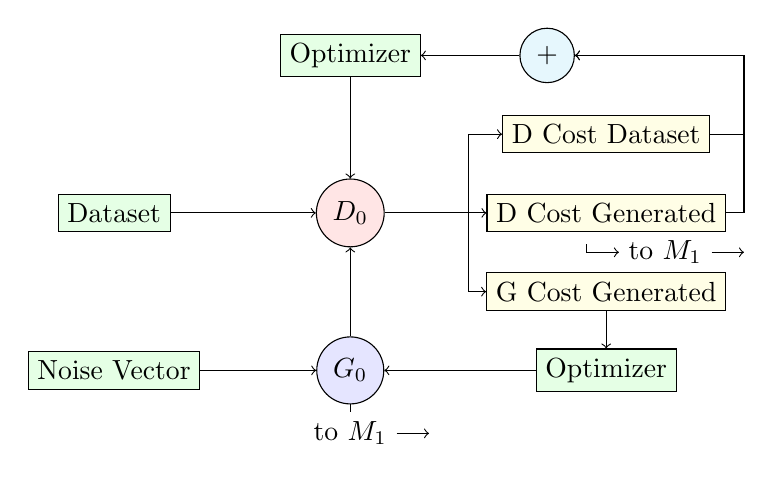
\begin{tikzpicture}
%style for generator node
\tikzstyle{gnode} = [circle, fill=blue!10, draw=black]

%style for discriminator node
\tikzstyle{dnode} = [circle, fill=red!10, draw=black]

%style for input box
\tikzstyle{inbox} = [rectangle, fill=green!10, draw=black]

%style for cost 
\tikzstyle{cost} = [rectangle, fill=yellow!10, draw=black]

%style for operator 
\tikzstyle{operator} = [circle, fill=cyan!10, draw=black]

%place nodes
\node[inbox] (noise) at (0,0) {Noise Vector};

\node[inbox] (dataset) at (0,2) {Dataset};

\node[gnode](generator) at (3,0) {$G_{0}$};

\node(gIToNext) at (3,-0.8) {to $M_{1}$}; 

\node[inbox] (gOptimizer) at (6.25, 0) {Optimizer};

\node[dnode](discriminator) at (3,2) {$D_{0}$};

\node[inbox] (dOptimizer) at (3,4) {Optimizer};

\node[cost] (dCostDataset) at (6.25,3){D Cost Dataset};

\node[cost] (dCostGenerated) at (6.25,2){D Cost Generated};
\node (dItoNext) at (7.0, 1.5){to $M_{1}$};

\node[cost] (gCostGenerated) at (6.25,1){G Cost Generated};

\node[operator] (adder) at (5.5,4){+};

\draw[->] (noise) -- (generator);

\draw[->] (generator) -- (discriminator) ;
\draw[->] (generator) -- (gIToNext) -- (4,-0.8);

\draw[->] (gOptimizer) -- (generator);

\draw[->] (gCostGenerated) -- (gOptimizer);

\draw[->] (dataset) -- (discriminator);

\draw[->] (discriminator) -- (4.5, 2) |- (dCostDataset);
\draw[->] (discriminator) -- (4.5,2) |- (gCostGenerated);
\draw[->] (dCostGenerated) (6.0,1.6) |- (6.0,1.5) |- (dItoNext);
\draw[->] (dItoNext) -- (8,1.5);

\draw[->] (discriminator) -- (dCostGenerated);

\draw[->] (dCostGenerated) -- (8,2) |- (adder);
\draw[->] (dCostDataset) -- (8,3) |- (adder);

\draw[->] (adder) -- (dOptimizer);

\draw[->] (dOptimizer) -- (discriminator);
\end{tikzpicture}
\caption{Chained GANs base Model, $M_{0}$}
\label{figCGANBase}
\end{figure}

As noted in the discussion of our high-level architecture, the first model of
the chained generative adversarial network feeds noise vectors as inputs to 
the generator of the generative adversarial network in $M_{0}$.  We represent
this with the box labeled, "Noise vector," in the lower left hand side of figure
\ref{figCGANBase} above, and the reader should take this as the starting point
when perusing this diagram.  We pass the noise vector as the input value for
the predict function Keras provides for neural networks, which in this case is 
the generator, $G_{0}$.  This allows us to get an output value from the
generator $G_{0}$, without changing any parameters of the generator $G_{0}$
neural network.  We are now following the arrow emanating from the top of
$G_{0}$ going to $D_{0}$ in the diagram above.  Also, note that there is a second 
arrow pointing into the neural network $D_{0}$ that indicates $D_{0}$ is getting
input from a dataset.  The discriminator of a generative adversarial network
generally receives inputs from two sources: the first source is the generator,
$G_{0}$ in this case, and the second is some dataset, which in this work is the
MNIST dataset.  For neural networks, Keras defines a train\_on\_batch function
requires at least two inputs, which are the input values for training, along
with the expected output values for each particular input value.  For the
discriminator $D_{0}$ of our first generative adversarial network $M_{0}$
pictured above, invoke the train\_on\_batch function of $D_{0}$ twice.   Once
where we give the output of $G_{0}$ as input to $D_{0}$, and the expected value 
of 0 for every generated output from $G_{0}$ because we wish to train $D_{0}$ to 
give an output of $0$, which represents a probability of $0$ that the output of
the generator $G_{0}$ could have come from the dataset, which is the MNIST
dataset in our work.  Calling the discriminator $D_0$'s train\_on\_batch
function with the output of the generator $G_{0}$ and $0$ as input values has
the side effect of optimizing $D_{0}$ for one training step, and the resulting
output value of this train\_on\_batch function will be the value of the loss
function the Keras library computes when optimizing the discriminator $D_{0}$.
We make a similar call to the discriminator $D_{0}$'s train\_on\_batch function 
but we use a batch of instances of the MNIST dataset, and expected values of all
$1$'s for the input value of train\_on\_batch because now we wish to train the
discriminator to output values of $1$ whenever it has an input from the genuine
dataset.  In this work an input of the genuine dataset would be an image from
the MNIST dataset.  Finally, we calculate a third cost used in training the
generator, but the manner this is done is somewhat circuitous and roundabout.
One should notice in the lower right-hand side of figure \ref{figCGANBase} the
box labeled, "G Cost Generated," We compute this cost from the discriminator
$D_{0}$ again, but we take advantage of the Keras library by defining a Model
that is comprised of $D_{0}$, and $G_{0}$ where we specify that the $D_{0}$
component is not trainable.  Then we invoke the train\_on\_batch function of
this model, which for our purposes is presently labeled $M_{0}$, which starts
the process from generating a batch of 32 $28\times28$ fake images out of noise
vectors using generator $G_{0}$, and so on, leading up to $D_{0}$ finally
outputting a value of a loss function. Note that in the code that accompanies
this work \cite{jhcgan}, as well as in the original code by E. Linder-Nor\'en
that models such as $M_{0}$ depicted above are named as variables that start
with the word, ``combined,'' in the variable name.

This concludes our discussion of the basic generative adversarial network that
serves as the building block for the system that is the 
chained generative adversarial network  we discuss in this work.  Now we move on
to the slightly different architecture of the successive models that constitute
the remainder of the chained generative adversarial network.  Please see the
digram in figure \ref{figCGANSucc}.

% diagram of successor GAN
\begin{figure}[htpb]
\begin{tikzpicture}
%style for generator node
\tikzstyle{gnode} = [circle, fill=blue!10, draw=black]

%style for discriminator node
\tikzstyle{dnode} = [circle, fill=red!10, draw=black]

%style for input box
\tikzstyle{inbox} = [rectangle, fill=green!10, draw=black]

%style for cost 
\tikzstyle{cost} = [rectangle, fill=yellow!10, draw=black]

%style for operator 
\tikzstyle{operator} = [circle, fill=cyan!10, draw=black]

%place nodes
\node[inbox] (gPrevOut) at (0,0) {$\mathcal{G}_{i-1}$ Output};

\node[inbox] (dataset) at (0,2) {Dataset};

\node[gnode](generator) at (3,0) {$G_{i}$};

\node(gIToNext) at (3,-0.8) {to $M_{i+1}$}; 
\node[inbox] (gOptimizer) at (6.25, 0) {Optimizer};

\node[dnode](discriminator) at (3,2) {$D_{i}$};

\node[inbox] (dOptimizer) at (3,4) {Optimizer};

\node[cost] (dCostDataset) at (6.25,3){D Cost Dataset};

\node[cost] (dCostGenerated) at (6.25,2){D Cost Generated};

\node (dItoNext) at (7.0, 1.5){to $M_{i+1}$};

\node[cost] (gCostGenerated) at (6.25,1){G Cost Generated};

\node[operator] (adder) at (5.5,4){+};

\draw[->] (noise) -- (generator);

\draw[->] (generator) -- (discriminator) ;
\draw[->] (generator) -- (gIToNext) -- (4,-0.8);

\draw[->] (gOptimizer) -- (generator);

\draw[->] (gCostGenerated) -- (gOptimizer);

\draw[->] (dataset) -- (discriminator);

\draw[->] (discriminator) -- (4.5, 2) |- (dCostDataset);
\draw[->] (discriminator) -- (4.5,2) |- (gCostGenerated);
\draw[->] (dCostGenerated) (6.0,1.6) |- (6.0,1.5) |- (dItoNext);
\draw[->] (dItoNext) -- (8,1.5);
\draw[->] (discriminator) -- (dCostGenerated);

\draw[->] (dCostGenerated) -- (8,2) |- (adder);
\draw[->] (dCostDataset) -- (8,3) |- (adder);

\draw[->] (adder) -- (dOptimizer);

\draw[->] (dOptimizer) -- (discriminator);
\end{tikzpicture}
\caption{Chained GANs successor model $M_{i}$}
\label{figCGANSucc}
\end{figure}

As one can surmise from the similarities in figures \ref{figCGANSucc}, and 
\ref{figCGANBase} there is not much functional difference between the generative
adversarial networks that constitute the models $M_{0}$, and the subsequent
models $M_{1}$, $M_{2}$, \ldots $M_{n}$. The key difference is the input to the
generator, depicted as $G_{i}$ above.  The input to the generator is now the
value of the $\mathcal{G}$ function that we describe in the commentary on the
high level functioning of the chained generative adversarial network that
accompanies figure \ref{figCGANHigh}.  Otherwise the functioning of the
generative adversarial networks that comprise models $M_{1}$, $M_{2}$, \ldots
$M_{n}$ is the same.

Now we move on to discuss the internals of the discriminators in our chained
generative adversarial networks.

% diagram for discriminator nodes
\begin{figure}[htpb]
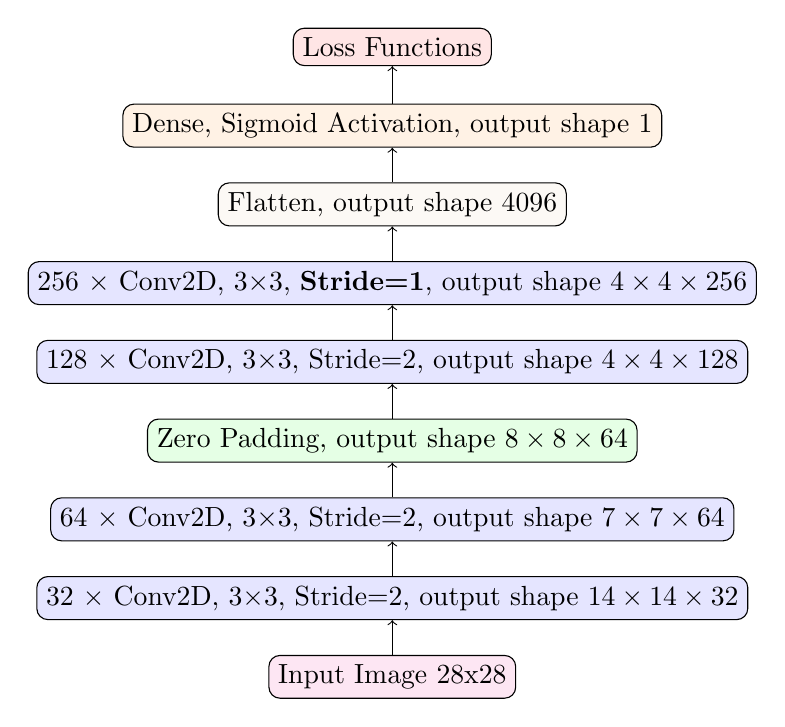
\begin{tikzpicture}
\tikzstyle{convlayer1} = [rectangle, rounded corners,fill=blue!10, draw=black]
\tikzstyle{zeropadding} = [rectangle, rounded corners,fill=green!10, draw=black]
\tikzstyle{outputshape} = [rectangle, rounded corners, fill=red!10, draw=black]
\tikzstyle{dropout} = [rectangle, rounded corners,fill=black!5, draw=black]
\tikzstyle{flatten} = [rectangle, rounded corners,fill=brown!5, draw=black]
\tikzstyle{optimizer} = [rectangle, fill=purple!5, draw=black]
\tikzstyle{loss} = [rectanble, fill=cyan!10, draw=black]
\tikzstyle{dense} = [rectangle, rounded corners, fill=orange!10, draw=black]
\tikzstyle{image} = [rectangle, rounded corners, fill=magenta!10, draw=black]

\node(inputImage) [image] at (0,0) {Input Image 28x28};
\node(convLayer1) [convlayer1] at (0,1) {32 $\times$ Conv2D, 3$\times$3,
  Stride=2, output shape $14 \times 14 \times 32$};
\node(convLayer2) [convlayer1] at (0, 2) {64 $\times$ Conv2D, 3$\times$3,
  Stride=2, output shape $7 \times 7 \times 64$};
\node(zeropad) [zeropadding] at (0,3) {Zero Padding, output shape 
  $8 \times 8 \times 64$};
\node(convLayer3) [convlayer1] at (0, 4) {128 $\times$ Conv2D, 3$\times$3,
  Stride=2, output shape $4 \times 4 \times 128$};
\node(convLayer4) [convlayer1] at (0, 5) {256 $\times$ Conv2D, 3$\times$3,
\textbf{Stride=1}, output shape $4 \times 4 \times 256$};
\node(flatten)[flatten] at (0,6) {Flatten, output shape 4096};
\node(dense) [dense] at (0,7) {Dense, Sigmoid Activation, output shape 1};
\node(sigmoid) [outputshape] at (0,8) {Loss Functions};
\draw[->] (inputImage) -- (convLayer1);
\draw[->] (convLayer1) -- (convLayer2);
\draw[->] (convLayer2) -- (zeropad);
\draw[->] (zeropad) -- (convLayer3);
\draw[->] (convLayer3) -- (convLayer4);
\draw[->] (convLayer4) -- (flatten);
\draw[->] (flatten) -- (dense);
\draw[->] (dense) -- (sigmoid);
\end{tikzpicture}
\caption{Discriminator architecture}
\label{discArch}
\end{figure}

The discriminators $D_{0}$, $D_{1}$, \ldots $D_{n}$ in a chained generative 
adversarial network are convolutional neural networks.  For our work, because we
rely so heavily on the Keras library, the Keras Conv2D function is critical to
the functioning of the discriminator.  The input layer
of the discriminator takes batch of 32 $28\times28$ images and performs a
32 convolutions (one for each filter) that result in a batch of 32 $14\times14$
arrays.  The output size is cut in half from $28\times28$ to $14\times14$ by
dint of using a stride value of two.  The next layer of the discriminator is a
similar convolution that cuts the outupt to a batch of $7\times7$ arrays.  Note
that we must use Keras' ZeroPadding layer functionality in order to continue -
this results in a batch of $8\times8$ arrays that are easier to then generate
smaller feature maps from as we proceed with convolutions.  Finally we flatten
the feature maps to a 4,096 element dense layer with a sigmoid activation
function.  It is the output of this sigmoid activation function that we
interpret as the probability that the discriminiators $D_{0}$, $D_{1}$, \ldots,
$D_{n}$ give that its input is a genuine instance of a dataset.  It is most
important for the reader to note that we omit some layers in the digram for the
discriminators of the chained generative adversarial networks in order to keep
the diagram to a manageable size.  Following every convolutional layer in the
neural networks that constitute the discriminators, we have a leaky rectified
linear unit (LeakyReLU) layer that serves as the activation function for that
layer.  In our work, we use the hyperparameter $\alpha$ value of $0.2$ for the
LeakyRelU layers.  Also accompanying every convolutional layer except the first
convolutional layer is a batch
normalization layer that we apply before the LeakyReLU layer.  Batch
normalization refers to the process of rescaling the output of the convolutional
layer so that all values have zero mean and unit variance.  Radford, Metz, and
Chintala write in \cite{repLearnDcgan} that this practice has the effect of stabilizing learning.
Finally after each LeakyReLU layer we have a dropout layer that is also not
pictured in the diagram above, but is nevertheless a used multiple times in the
discriminators. While the authors of \cite{repLearnDcgan} do not mention using any
dropout layers, we note that Goodfellow \textit{et al.} recommend using dropout
in \cite{deepLearnBookGenCh} where they write, ``Dropout seems to be important
in the discriminator network.''  We take this as the reason that E.
Linder-Nor\'en uses dropout layers in \cite{kerasdcgan}, and we use his Keras
implemenation of deep convolutional generative adversarial networks as the basis
for our chained generative adversarial networks. 

This concludes our discussion of the discriminator portion of the models of the
chained generative adversarial network system, and we move on to give the
details of the generators.  Please see the diagram in figure \ref{genArch}
below, and the commentary that accompanies it.
% diagram for generator nodes
\begin{figure}[htpb]
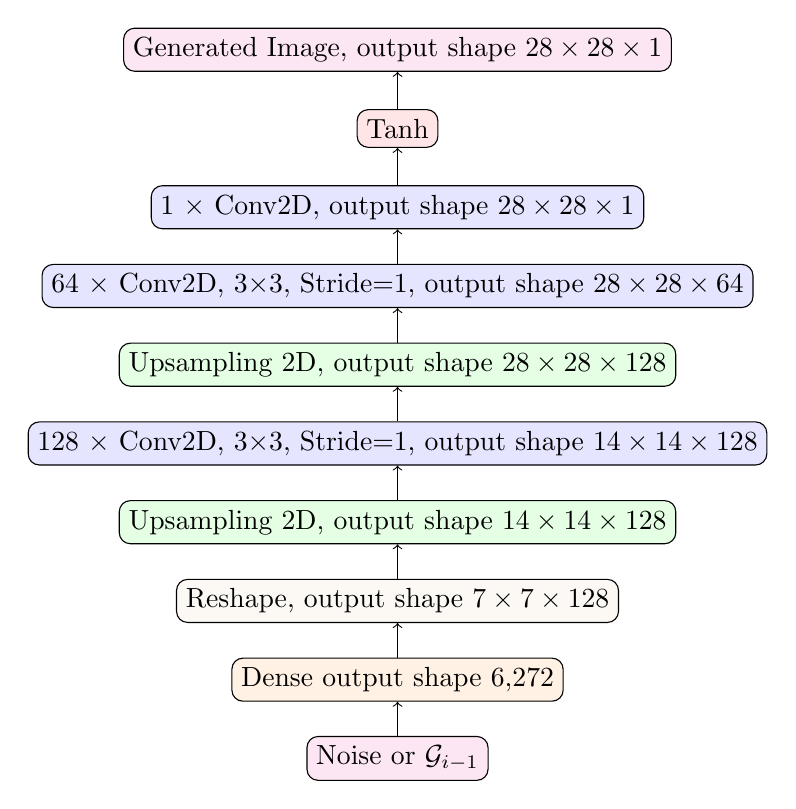
\begin{tikzpicture}
\tikzstyle{convlayer1} = [rectangle, rounded corners,fill=blue!10, draw=black]
\tikzstyle{upsampling} = [rectangle, rounded corners,fill=green!10, draw=black]
\tikzstyle{outputshape} = [rectangle, rounded corners, fill=red!10, draw=black]
\tikzstyle{dropout} = [rectangle, rounded corners,fill=black!5, draw=black]
\tikzstyle{flatten} = [rectangle, rounded corners,fill=brown!5, draw=black]
\tikzstyle{optimizer} = [rectangle, fill=purple!5, draw=black]
\tikzstyle{loss} = [rectanble, fill=cyan!10, draw=black]
\tikzstyle{dense} = [rectangle, rounded corners, fill=orange!10, draw=black]
\tikzstyle{image} = [rectangle, rounded corners, fill=magenta!10, draw=black]

\node(inputImage) [image] at (0,0) {Noise or $\mathcal{G}_{i-1}$};
\node(dense) [dense] at (0,1) {Dense output shape 6,272};
\node(reshape)[flatten] at (0,2) {Reshape, output shape $7\times7\times128$};
\node(upsample1) [upsampling] at (0,3) {Upsampling 2D, output shape
$14\times14\times 128$};
\node(convLayer1) [convlayer1] at (0,4) {128 $\times$ Conv2D, 3$\times$3,
  Stride=1, output shape $14 \times 14 \times 128$};
\node(upsample2) [upsampling] at (0,5) {Upsampling 2D, output shape
$28\times28\times128$};
\node(convLayer2) [convlayer1] at (0, 6) {64 $\times$ Conv2D, 3$\times$3,
  Stride=1, output shape $28 \times 28 \times 64$};
\node(convLayer3) [convlayer1] at (0,7) {1 $\times$ Conv2D, output shape 
  $28 \times 28 \times 1$};
\node(tanh) [outputshape] at (0,8) {Tanh};
\node(outputImg) [image] at(0,9) {Generated Image, output shape
  $28 \times 28 \times 1$};
\draw[->] (inputImage) -- (dense);
\draw[->] (dense) -- (reshape);
\draw[->] (reshape) -- (upsample1);
\draw[->] (upsample1) -- (convLayer1);
\draw[->] (convLayer1) -- (upsample2);
\draw[->] (upsample2) -- (convLayer2);
\draw[->] (convLayer2) -- (convLayer3);
\draw[->] (convLayer3) -- (tanh);
\draw[->] (tanh) -- (outputImg);
\end{tikzpicture}
\caption{Generator architecture}
\label{genArch}
\end{figure}

The generators of the chained generative adversarial network system share a
common architecture, the main difference between any of them is that which we
highlighted above.  This is the difference that the first generator uses vectors
of random noise for input, whereas subsequent generators use the augmented
output of the previous generators via the $\mathcal{G}$ function we described
above.  

Each generator begins with a batch of vectors that we feed to a dense layer.
The first generator will use a a batch of random valued vectors where the values
are drawn from the normal distribution on $\left(0, 1\right)$. Otheriwse the
input to the first layer of the generator will be a vector with elements that
are the values of the $\mathcal{G}$ function.  Regardless of how we obtain this
input, in all the generators we feed this to a dense network that we reshape 
to a batch of $7\times7\times128$ feature maps and feed to subsequent upsampling
and convolutional layers.  Convolutional layers are necessary so that we have
trainable parameters, and we require upsampling to expand feature maps into
arrays large enough that we can interpret as fictitious instances of some
dataset. In order to keep the diagram to a manageable size we omit relu
activations in every layer except the final layer, which we expliclitly depict
as a tanh layer in the diagram above.  Radford, Metz and Chintala explain that
we use a tanh activation in the output layer in order that we may more easily
interpret the output of the generator as an image in \cite{repLearnDcgan}. 

Finally, to further elucidate the architecture of the chained generative
adversarial network system, we present a section of pseudocode that summarizes
the training steps of the components of the system.

We give pseudocode for the key training steps of the CGAN's below.  Please 
keep in mind the following definitions and notations when reading the pseudocode:
\begin{itemize}
\item a model $M_{i}$ is a system of two neural networks $D_{i}$ and $G_{i}$. We
codify this relationship with the notation $M_{i}=\left(G_{i},D_{i}\right)$.
Model and GAN are synonyms.
\item This work covers systems of generators and discriminators (models) that
are ordered in the sense that successor models use the output of predecessor
models for their inputs.  Hence $D_{0}$ is the first discriminator, and $G_{0}$
is the first generator.  $D_{i}$ is a successor discriminator, and $G_{i}$ is
a successor generator. $D_{n}$, and $G_{n}$, are the last discriminator, and
generator, respectively.
\item The entire collection of models (GAN's) is $\mathbf{M}$.
\item $\mathbf{Z}$ is a list of vectors $\hat{\mathbf{z}}_{i}$, where the components 
of each $\hat{\mathbf{z}}_{i}$ is a random number sampled from the normal 
distribution on $\left(0,1\right)$.
\item $G_{0}\left(\mathbf{Z}\right)$ is the output of the zeroth generator
$G_{0}$ for the input values of $\mathbf{Z}$.
\item $D_{0}\left(G_{0}\right)$ is the output of the zeroth discriminator for
the input value of $G_{0} = G_{0}\left(\mathbf{Z}\right)$.
\item $\mathbf{X}$ is a list of instances of a dataset $\mathbf{S}$.  In GAN's the
discriminator is a classifier that attempts to label its inputs as either
genuine instances of $\mathbf{S}$ or synthetic imposters that some generator has
created.  In the code that accompanies this work, $1$ is the desired
output value of the discriminator if it is given an element of $\mathbf{X}$ as
an input value, and $0$ is the desired output value of the discriminator if it
is given the output value of some generator as an input value.
\item $L\left(D_{i}\left(\mathbf{X}\right)\right)$ is the loss function the
model $M_{i}$ (GAN) uses in conjunction with the optimizer for the output value of a 
discriminator $D_{i}$ for input values $\mathbf{X}$.
\item $L\left(D_{i}\left(G_{i}\right)\right)$ is the loss function evaluated
on the output of discriminator $D_{i}$ when $D_{i}$ uses the output of $G_{i}$
as input.
\item $L\left(M_{i}\right)$ is the value of the loss function of with the value
of the combined model $M_{i}=\left(G_{i}, D_{i}\right)$.  In our code, we train a
combined model to update the generator, however, in that combined model the
discriminator is configured to be \textbf{not} trainable.  Therefore the
optimizer only updates the generator component of the GAN during the portion of
training where the generator is trained.
\item $\mathcal{G}_{i} = \mathcal{G}\left(G_{i-1},  
L\left(D_{i-1}\left(G_{i-1}\right)\right)\right)$ is
the input for generator $G_{i}$ that we calculate as the function
$\mathcal{G}$ that flattens the output of $G_{i-1}$ to 1-dimensional array,
and then concatenates the value of the loss function
$L\left(D_{i-1}\left(G_{i-1}\right)\right)$ to it. One should keep this in mind
in contrast with the vectors of random numbers $\mathbf{Z}$ that are the input
values for the first generator, $G_{0}$.
\end{itemize}

Please  see the pseudocode labeled \ref{trainalg} for the pseudocode for the 
training step of the chained GAN's.  The pseudocode utilizes all the notation
in the previous list.

\begin{algorithm}[htpb]
 \KwData{Inputs: $\mathbf{Z}$, $\mathbf{X}$}
 \KwResult{Trained system of GAN's $\mathbf{M}$}
 initialization\;
 use standard Keras layer components to instantiate $n$ identical generator neural
 networks $G_{0}$, $G_{1}$, \ldots, $G_{n}$\;
 use standard Keras layer components to instantiate $n$ identical discriminator neural
networks $D_{0}$, $D_{1}$, \ldots, $D_{n}$\;
 create combined models $M_{0}$, $M_{1}$, \ldots, $M_{n}$ such that
$M_{i}=\left(G_{i},D_{i}\right)$\;
 \For{number of epochs}{
note: Keras \textit{train batch} function has the side effect of updating the neural
network's trainable parameters\;
  $L\left(D_{0}\left(G_{0}\right)\right), D_{0}\left(G_{0}\right) \leftarrow \text{train batch}
    \left(D_{0}\left(G_{0}\left(\mathbf{Z}\right)\right)\right)$\;

  $L\left(D_{0}\left(\mathbf{X}\right)\right) \leftarrow \textit{train batch}
    \left(D_{0}\left(\mathbf{X}\right)\right)$\;

  $L\left(M_{0}\right) \leftarrow \textit{train batch}\left(M_{0}\right)$\;
  \For{i = 1 to number of successor GAN's}{
      $\mathcal{G}_{i} \leftarrow \mathcal{G}\left(G_{i-1}, 
        L\left(D_{i-1}\left(G_{i-1}\right)\right)\right)$\;
   
     $L\left(D_{i}\left(G_{i}\right)\right), D_{i}\left(G_{i}\right) \leftarrow \text{train batch}
         \left(D_{i}\left(G_{i}\left(\mathcal{G}_{i-1}\right)\right)\right)$\;
     
     $L\left(D_{i}\left(\mathbf{X}\right)\right) \leftarrow \textit{train batch}
       \left(D_{i}\left(\mathbf{X}\right)\right)$\;
   
     $L\left(M_{i}\right) \leftarrow \textit{train batch}\left(M_{i}\right)$\;
   } 
  }
 \caption{Pseudocode for chained GAN's training steps}
\label{trainalg}

\end{algorithm}

We hope the reader has a clear idea of the functioning of the chained generative
adversarial network system at its various levels.  We now move on to discuss the
experiments we perform with this system.

\section{Experiments}

The main purpose of the experiments we perform is to investigate the behavior of
the generators and discriminators in the chained generative adversarial network
system as the output of the generators flows through the system.  Specifically
we wish to know how the accuracy and the loss changes when we look at values of 
these metrics for the generator $G_{0}$, discriminator $D_{0}$, and subsequent
generators and discriminators $G_{1}$, $D_{1}$, and so on.

The tools we use to conduct the experiments we report on below are as follows.
We started with the python code in \cite{kerasdcgan} from Github.  We then
forked this code and modified it to the architecture we present in the previous
section.  In addition, we incorporated a Tensorflow tensorboard callback
function to facilitate recording the data we report below.  In order to get a
feel for the repeatability of the results, we conducted 3 trials. We compiled
the latest tensorflow source code using commit
a49887b0d24c9c1a97c5915147473bb09f854ebc from November 25th.  We compiled this
version of tensorflow specifically for a g3s.xlarge Amazon Web Services EC2
instance to take advantage of the Nvidia Tesla M-60 GPU that Amazon includes
with g3s instances.  In addition we the AWS g3s instance we used runs Ubuntu
version 16, and we use the instructions in \cite{tensorflowbuild} in order to 
compile tensorflow from source.  In order to modify the code in
\cite{kerasdcgan} to achieve our implementation, we used the Pycharm integrated 
development environment.  

The baseline method is the behavior of the first generative adversarial network 
in the chained generative adversarial network system.  The output of the
generators is most instructive in describing the functionality of the base
system.  For these experiments, the output is images that resemble MNIST images.
First, consider the output of the untrained generative adversarial network. The
image below is from the Keras implementation of Radford, Metz, and Chintala's
deep convolutional generative adversarial networks, from \cite{kerasdcgan}.
\begin{figure}[htbp]
\centerline{\includegraphics[scale=0.5]{chain-gan-images/2018-12-07/0900/mnist_generator_0_0.png}}
\caption{First output of base model generated images}
\label{initalGan}
\end{figure}

Note how in the image above, the images resemble static on television screens
because they are images with random greyscale values as pixels.  The next image
shows the behavior of the base model after convergence. Note that the images now
appear to be more organized, and they resemble handwritten digits:
 \begin{figure}[htbp]
\centerline{\includegraphics[scale=0.5]{chain-gan-images/2018-12-07/0900/mnist_generator_0_1750.png}}
\caption{Epoch 1,750 output of base model generated images}
\label{trainedBaseGan}
\end{figure}


We give the images of the output of the baseline system, which is the Keras
implementation of the deep convolutional generative adversarial network from
\cite{kerasdcgan}, to emphasize the functionality of the code we copy as a
starting point for our work.  It clearly defines a deep convolutional generative
adversarial network with a tangible result of a progression of generated images
that start off as noise, and progress to images that closely resemble images of
the MNIST dataset, which is what the generative adversarial network in
\cite{kerasdcgan} is designed to generate.  

The performance measures we look at for our experiments are: accuracy of the
generators and discriminators, and the value of the loss functions for the
generators and the discriminators.  We leave it as a topic for future work to
include more metrics.

In order to conduct our experiments we extend the baseline of 4,000 epochs to
8,000 epochs to attempt to detect if the chaining of the output of subsequent
generators has some instability that that the baseline system does not
encounter.

For our experiments we fix the number of generative adversarial networks in the 
system of chained generative adversarial networks at 6.  We have one baseline 
generative adversarial network, chained to 5 successive generative adversarial
networks $M_{1}$, through $M_{5}$.  Thus the first generative adversarial
network embodied in $M_{0}$ has generator $G_{0}$, and discriminator $D_{0}$,
and so on.

First of all we show the performance measures for the baseline system.  The
loss function for generators of the baseline system is as follows:

\begin{figure}[htpb]
\begin{tikzpicture}
\begin{axis}
\addplot table [x=Step, y=Value, col sep=comma, mark options={black}, 
  only marks]
{./tensorboard-data/2018-12-07/0900/csv/run-0900-tag-Generator-0-Loss.csv};
\legend{Loss}
\end{axis}
\end{tikzpicture}
\caption{Baseline generator loss, x-axis is epoch number, y-axis is 
value of binary cross entropy loss function }
\label{gen0Loss}
\end{figure}

We see the expected behavior that the generator trains to quickly minimize the
value of its loss function, and then subsequently the value of the loss function
hovers randomly in a narrow range.

The loss functions of the chain of generative adversarial networks that we give
the architecture for in the previous section are in the charts below:

\begin{figure}[htpb]
\begin{tikzpicture}
\begin{axis}
\addplot table [x=Step, y=Value, col sep=comma, mark options={black}, 
  only marks]
{./tensorboard-data/2018-12-07/0900/csv/run-0900-tag-Generator-1-Loss.csv};
\legend{Loss}
\end{axis}
\end{tikzpicture}
\caption{generator $G_{1}$ loss, x-axis is epoch number, y-axis is 
value of binary cross entropy loss function }
\label{gen1Loss}
\end{figure}

\begin{figure}[htpb]
\begin{tikzpicture}
\begin{axis}
\addplot table [x=Step, y=Value, col sep=comma, mark options={black}, 
  only marks]
{./tensorboard-data/2018-12-07/0900/csv/run-0900-tag-Generator-2-Loss.csv};
\legend{Loss}
\end{axis}
\end{tikzpicture}
\caption{generator $G_{2}$ loss, x-axis is epoch number, y-axis is 
value of binary cross entropy loss function }
\label{gen2Loss}
\end{figure}

\begin{figure}[htpb]
\begin{tikzpicture}
\begin{axis}
\addplot table [x=Step, y=Value, col sep=comma, mark options={black}, 
  only marks]
{./tensorboard-data/2018-12-07/0900/csv/run-0900-tag-Generator-3-Loss.csv};
\legend{Loss}
\end{axis}
\end{tikzpicture}
\caption{generator $G_{3}$ loss, x-axis is epoch number, y-axis is 
value of binary cross entropy loss function }
\label{gen3Loss}
\end{figure}

\begin{figure}[htpb]
\begin{tikzpicture}
\begin{axis}
\addplot table [x=Step, y=Value, col sep=comma, mark options={black}, 
  only marks]
{./tensorboard-data/2018-12-07/0900/csv/run-0900-tag-Generator-4-Loss.csv};
\legend{Loss}
\end{axis}
\end{tikzpicture}
\caption{generator $G_{4}$ loss, x-axis is epoch number, y-axis is 
value of binary cross entropy loss function }
\label{gen4Loss}
\end{figure}

\begin{figure}[htpb]
\begin{tikzpicture}
\begin{axis}
\addplot table [x=Step, y=Value, col sep=comma, mark options={black}, 
  only marks]
{./tensorboard-data/2018-12-07/0900/csv/run-0900-tag-Generator-5-Loss.csv};
\legend{Loss}
\end{axis}
\end{tikzpicture}
\caption{generator $G_{5}$ loss, x-axis is epoch number, y-axis is 
value of binary cross entropy loss function }
\label{gen5Loss}
\end{figure}

We find nothing interesting in the successive generator's accuracies in
figures \ref{gen1Loss} through \ref{gen5Loss}.  They
resemble scatter plots of random values ranging from 2 to 6.  However we see
there is some compelling reason why this may be the case, the generators appear
to flail around randomly because the discriminators are able to give accurate
probabilities that their input data is genuine data from a dataset, and the
generators are unable to learn to fool the discriminators as they should be in
the convergence state that Goodfellow \textit{et al.} describe in \cite{gan}.

First we report the performance of the baseline discriminator loss function and
accuracy:

\begin{figure}[htpb]
\begin{tikzpicture}
\begin{axis}
\addplot table [x=Step, y=Value, col sep=comma, mark options={black}, 
  only marks]
{./tensorboard-data/2018-12-07/0900/csv/run-0900-tag-Discriminator-0-Loss.csv};
\legend{Loss}
\end{axis}
\end{tikzpicture}
\caption{Baseline discriminator $D_{0}$ loss, x-axis is epoch number, y-axis is 
value of binary cross entropy loss function }
\label{disc0Loss}
\end{figure}

Again as in the case with the generator, in figure \ref{disc0Loss} we see that the 
discriminator's loss function starts high and then quickly converges to a stable 
value.  

Next we look at the accuracy of the baseline discriminator network.

\begin{figure}[htpb]
\begin{tikzpicture}
\begin{axis}
\addplot table [x=Step, y=Value, col sep=comma, mark options={black}, 
  only marks]
{./tensorboard-data/2018-12-07/0900/csv/run-0900-tag-Discriminator-0-Accuracy.csv};
\legend{Accuracy}
\end{axis}
\end{tikzpicture}
\caption{Baseline discriminator $D_{0}$ accuracy, x-axis is epoch number, y-axis is 
percentage of correctly classified input values }
\label{disc0Acc}
\end{figure}

In figure \ref{disc0Acc} we see the result Goodfellow \textit{et al.} predict in
\cite{gan}; the discriminator accuracy resembles a scatterplot of random values
around the 60\% mark.  This is because the generator learns to fool the
discriminator and the discriminator can do no better than give about a 0.5
probability that the input it is given is coming from a real dataset versus from
a generator, in this case it is the generator $G_{0}$ we discuss above.

Now we move on to look at the plots for
the subsequent discriminators $D_{1}$ through $D_{5}$:

\begin{figure}[htpb]
\begin{tikzpicture}
\begin{axis}
\addplot table [x=Step, y=Value, col sep=comma, mark options={black}, 
  only marks]
{./tensorboard-data/2018-12-07/0900/csv/run-0900-tag-Discriminator-1-Loss.csv};
\legend{Loss}
\end{axis}
\end{tikzpicture}
\caption{Baseline discriminator $D_{1}$ loss, x-axis is epoch number, y-axis is 
value of binary cross entropy loss function }
\label{disc1Loss}
\end{figure}

\begin{figure}[htpb]
\begin{tikzpicture}
\begin{axis}
\addplot table [x=Step, y=Value, col sep=comma, mark options={black}, 
  only marks]
{./tensorboard-data/2018-12-07/0900/csv/run-0900-tag-Discriminator-1-Accuracy.csv};
\legend{Accuracy}
\end{axis}
\end{tikzpicture}
\caption{Discriminator $D_{1}$ accuracy, x-axis is epoch number, y-axis is 
percentage of correctly classified input values }
\label{disc1Acc}
\end{figure}

We note nothing important in figure \ref{disc1Loss}. However, we see that figure
\ref{disc1Acc} reflects a higher accuracy for the discriminator $D_{1}$.  We
move on to show charts for the accuracies  for the remaining discriminators
since we do not find anything interesting in the loss values for the remaining
discriminators.

\begin{figure}[htpb]
\begin{tikzpicture}
\begin{axis}
\addplot table [x=Step, y=Value, col sep=comma, mark options={black}, 
  only marks]
{./tensorboard-data/2018-12-07/0900/csv/run-0900-tag-Discriminator-2-Accuracy.csv};
\legend{Accuracy}
\end{axis}
\end{tikzpicture}
\caption{discriminator $D_{2}$ accuracy, x-axis is epoch number, y-axis is 
percentage of correctly classified input values }
\label{disc2Acc}
\end{figure}

\begin{figure}[htpb]
\begin{tikzpicture}
\begin{axis}
\addplot table [x=Step, y=Value, col sep=comma, mark options={black}, 
  only marks]
{./tensorboard-data/2018-12-07/0900/csv/run-0900-tag-Discriminator-3-Accuracy.csv};
\legend{Accuracy}
\end{axis}
\end{tikzpicture}
\caption{discriminator $D_{3}$ accuracy, x-axis is epoch number, y-axis is 
percentage of correctly classified input values }
\label{disc3Acc}
\end{figure}

\begin{figure}[htpb]
\begin{tikzpicture}
\begin{axis}
\addplot table [x=Step, y=Value, col sep=comma, mark options={black}, 
  only marks]
{./tensorboard-data/2018-12-07/0900/csv/run-0900-tag-Discriminator-4-Accuracy.csv};
\legend{Accuracy}
\end{axis}
\end{tikzpicture}
\caption{discriminator $D_{4}$ accuracy, x-axis is epoch number, y-axis is 
percentage of correctly classified input values }
\label{disc4Acc}
\end{figure}

\begin{figure}[htpb]
\begin{tikzpicture}
\begin{axis}
\addplot table [x=Step, y=Value, col sep=comma, mark options={black}, 
  only marks]
{./tensorboard-data/2018-12-07/0900/csv/run-0900-tag-Discriminator-5-Accuracy.csv};
\legend{Accuracy}
\end{axis}
\end{tikzpicture}
\caption{discriminator $D_{5}$ accuracy, x-axis is epoch number, y-axis is 
percentage of correctly classified input values }
\label{disc5Acc}
\end{figure}

We notice the conintued trend of higher accuracies for subsequent
discriminators. It also appears that there may be a greater percentage of
accuracy values captured that are closer to the top of the range.

Therefore we decided to repeat this experiment two more times, and compute
summary statitics of the accuracy values for the discriminators.  We export
the data that tensorboard captures while we run these experiments as csv files,
and report mean accuracy values along with the standard deviations of the
accuracy values, to give the reader an indication of the spread of these
accuracy values for each of the three trials we perform.

\begin{table}[htpb]
\begin{center}
\begin{tabular}{|c|c|c|c|}
  \hline
  Trial & Discriminator & Accuracy & Standard Deviation  \\\hline
  1 & 0 & 58.35 & 8.44    \\\hline
  1 & 1 & 89.91 & 8.63   \\\hline
  1 & 2 & 82.61 & 11.35   \\\hline
  1 & 3 & 87.38 & 10.37  \\\hline
  1 & 4 & 86.53 & 10.71   \\\hline
  1 & 5 & 88.42 & 10.41    \\\hline
  2 & 0 & 59.76 & 8.61    \\\hline
  2 & 1 & 91.62 & 8.65   \\\hline
  2 & 2 & 87.62 & 10.29   \\\hline
  2 & 3 & 88.0 & 11.38  \\\hline
  2 & 4 & 91.16 & 9.64   \\\hline
  2 & 5 & 92.13 & 9.58    \\\hline
  3 & 0 & 59.08 & 8.71    \\\hline
  3 & 1 & 90.90 & 8.83   \\\hline
  3 & 2 & 90.19 & 10.39   \\\hline
  3 & 3 & 90.03 & 9.95  \\\hline
  3 & 4 & 90.54 & 10.04   \\\hline
  3 & 5 & 92.76 & 9.34    \\\hline

  \end{tabular}
\caption{Mean Accuracy for Discriminators, non-baseline discriminator accuracy
is consistently higher}
\label{discTab}
\end{center}
\end{table}

We notice that the mean accuracy for the non-baseline discriminators  in table
\ref{discTab} is higher than 0.5.   This would indicate that the chained
discriminators are not confused about whether the output they are seeing is from
a generator, or a dataset.  The generators $G_{0}$ through $G_{5}$  produce
output in the same format, and the discriminators $D_{0}$ through $D_{5}$ get
input from either the respective generator or the dataset.  However, there seems
to be some observable effect happening that when the generators generate output
not from noise, but from some values based on the output of a previous
generator, that the discriminators are better able to classifiy their input as
either coming from a generator or coming from an actual dataset.

These emprical results support the statement in the previous pararagraph, but we
do not have a theory as to why this is the case at this time.

Finally, we pick a randomly chosen batch of images generated from the $M_{5}$
generative adversarial network to illustrate that, to the human viewer, the
output of the generative adversarial newtork is different or of noticably lower
quality than the images we see in \ref{trainedBaseGan}.

\begin{figure}[htbp]
\centerline{\includegraphics[scale=0.5]{chain-gan-images/2018-12-07/0900/mnist_generator_5_1750.png}}
\caption{Epoch 1,750 output of model $M_{5}$ generated images}
\label{trainedBaseGan}
\end{figure}


\section{Conclusions}

In this work we present an architecture for chaining generative adversarial
networks together.

The key to our implementation is to use the output of a basis generative
adversarial network that works along the lines of the deep convolutional
generative adversarial network that Radford, Metz, and Chintala give in
\cite{repLearnDcgan} as the input for similarly functioning generative
adversarial networks in an iterative fashion.

We devise a function that incorporates one of the values of the loss functions
that are typically computed to train the component generator and discriminator
of a generative adversarial network with the output of the generator of a
generative adversarial network, and we use the output of this function as a way
to tie successive members of a group of generative adversarial networks
together.

We report data from experiments that supports the hypothesis that when a
generator's input is not from a random source, but is the output of a generator
trained in a generative adversarial network to fit the same dataset, then the
discriminators in the successive generative adversarial networks are able to
identify instances of the dataset, versus generated instances with a higher
degree of accuracy.

Interestingly, the quality of output generated from the successive generative
adversarial networks that do not use random noise as inputs for the generators
does not appear to be of remarkably lower quality.  This implies that the
architecture we give is a stable method for linking multiple generative
adversarial networks together to perform some function.

We leave for future work the tasks of determining the repeatability of this work
over larger combinations of hyperparameters that we have fixed in the code in
\cite{jhcgan}, as well as assessing the repeatability of these results with
different baseline generative adversarial network components, as opposed to the
deep convolutional generative adversarial framework that we copy from Radford,
Metz and Chintala from \cite{repLearnDcgan}.  Another avenue of future research
is to gather additional metrics from the component generative adversarial
networks and see if other metrics follow some noticeable trend as discriminator
accuracy appears to follow in our results.  Finally, we offer no formal
justification for the increased accuracy of the discriminators that we observe,
therefore it is an important future work to find such a derivation should it
exist.

\section{References}

\begin{thebibliography}{00}

\bibitem{gan} I. Goodfellow \textit{et al.}, ``Generative Adversarial Nets,''
Neural Information Systems Processing Conference, 2014.  [Online]. Available:
\url{https://papers.nips.cc/paper/5423-generative-adversarial-nets.pdf}. [Accessed 
Dec. 2, 2018].
 
\bibitem{scargan} Lau \textit{et al.}, ``ScarGAN: Chained Generative Adversarial
  Networks to Simulate Pathological Tissue on Cardiovascular MR Scans,'' August
2018. Available:arXiv:1808.04500 [cs.CV], 
\url{https://arxiv.org/pdf/1808.04500v1.pdf}.  [Accessed November 12, 2018].

\bibitem{pix2pix} P. Isola, J.Y. Zhu, T. Zhou, and A. A. Efros, ``Image-to-Image
Translation with Conditional Adversarial Networks,'' Available:
arXiv:1611.07004 [cs.CV], \url{http://www.umi.com/proquest/}. [Accessed November
23, 2018].

\bibitem{repLearnDcgan} S. Chintala, L. Metz, and A. Radford,
Unsupervised representation learning with deep convolutional generative
adversarial networks.  2016. [Online]. Available: arXiv:1511.06434v2 [cs.LG]
\url{https://arxiv.org/pdf/1511.06434.pdf}. 

\bibitem{stackgan} Zhang \textit{et al.}, ``StackGAN: Text to Photo-realistic
Image Synthesis with Stacked Generative Adversarial Networks,'' August 2017. 
Available:  arXiv:1612.03242 [cs.CV] , \url{https://arxiv.org/pdf/1612.03242.pdf}.
[Accessed November 12, 2018].

\bibitem{galaxy} L. Fussell and B. Moews, ``Forging new worlds: high-resolution
synthetic galaxies with chained generative adversarial networks,'' 
December 2018. Available: arXiv:1811.03081 [astro-ph.IM],
\url{https://arxiv.org/pdf/1811.03081.pdf}.  [Accessed December 7, 2018].

\bibitem{kerasdcgan} E. Linder-Nor\'en, “Keras implementations of
Generative Adversarial Networks,” November, 2018.  [Online].
Available: \url{https://github.com/eriklindernoren/Keras-GAN}.
[Accessed December 1, 2018].

\bibitem{deepLearnBookGenCh} Y. Bengio, A. Courville, I. Goodfellow. (2016).
``Chapter 20 Deep Generative Models,'' 2016. [Online] Available:
\url{https://www.deeplearningbook.org/contents/generative\_models.html}.
[Accessed: November 20, 2018].

\bibitem{cgan} M. Mirza and S. Osindero, ``Conditional Generative Adversarial
Nets,'' November 2014. Available: arXiv:1411.1784 [cs.LG],
\url{https://arxiv.org/pdf/1411.1784.pdf}.  [Accessed November 17, 2018].

\bibitem{mnist} Y. LeCunn, C. Cortes and C. J.C. Burges, ``The MNIST Database of 
Handwritten Digits,'' yann.lecun.com. [Online]. Available:
\url{http://yann.lecun.com/exdb/mnist/} [Accessed Nov.  29, 2018].

\bibitem{lsgan} X. Mao, \textit{et al}., ``Least Squares Generative Adversarial 
Networks,'', April 2017. Available:   arXiv:1611.04076 [cs.CV],
\url{https://arxiv.org/pdf/1611.04076.pdf}.  [Accessed November 18, 2018].

\bibitem{jhcgan} J. Hancock., ``chain-gan.py'' December 2018. [Online].
Available:
\url{https://github.com/jhancock1975/Keras-GAN/blob/term/chain-gan/chain-gan.py}.
[Accessed December 10, 2018].

\bibitem{tensorflowbuild} Tensorflow.org, ``Build from source,''
 [Online].  Available: https://www.tensorflow.org/install/source. 
[Accessed: Nov. 12, 2018].

\bibitem{boltzmann} R. Salakhutdinovand and G. Hinton, ``Deep Boltzmann
Machines,'' Proceedings of the 12th International Confe-rence
on Artificial Intelligence and Statistics (AISTATS). 2009. Available:
\url{http://proceedings.mlr.press/v5/salakhutdinov09a/salakhutdinov09a.pdf}.
 [Accessed November 30, 2018].

\bibitem{varbayes} D. P. Kingma and M. Welling, ``Auto-Encoding Variational
Bayes'', May 2014.  Available   arXiv:1312.6114 [stat.ML]
\url{https://arxiv.org/pdf/1312.6114.pdf} [Accessed December 1, 2018]

\end{thebibliography}
\end{document}
